\documentclass[12pt,letterpaper]{article}
\usepackage[margin=0.7in,headheight=15pt,headsep=10pt,footskip=20pt]{geometry}
\usepackage[T1]{fontenc}
\usepackage{lmodern}
\usepackage{tikz}
\usetikzlibrary{arrows.meta}
\usepackage{fancyhdr}
\renewcommand{\familydefault}{\sfdefault}
\pagestyle{fancy}
\fancyhf{}
\fancyhead[L]{\fontsize{10.2}{12}\selectfont Week 4 / Stars-and-wheels return visits / Grades 2--5}
\fancyfoot[L]{\fontsize{9.2}{11}\selectfont Bellingham Math Circle / Week 4 / F04-RV-v1}
\fancyfoot[R]{\fontsize{9.2}{11}\selectfont\thepage}
\renewcommand{\headrulewidth}{0pt}
\renewcommand{\footrulewidth}{0pt}
\setlength{\parindent}{0pt}
\setlength{\parskip}{4pt}
\definecolor{counterred}{RGB}{169,43,42}
\definecolor{counterblue}{RGB}{36,83,160}
\tikzset{chip/.style={circle,draw,minimum size=7mm,inner sep=0pt,font=\small},
  arrow/.style={-{Stealth[length=2mm]},line width=.65pt}}

% All lengths below are physical millimetres, with equal x and y scale.
% The twelve working circles have diameter 21 mm and center radius 46 mm.
\newcommand{\workingring}{%
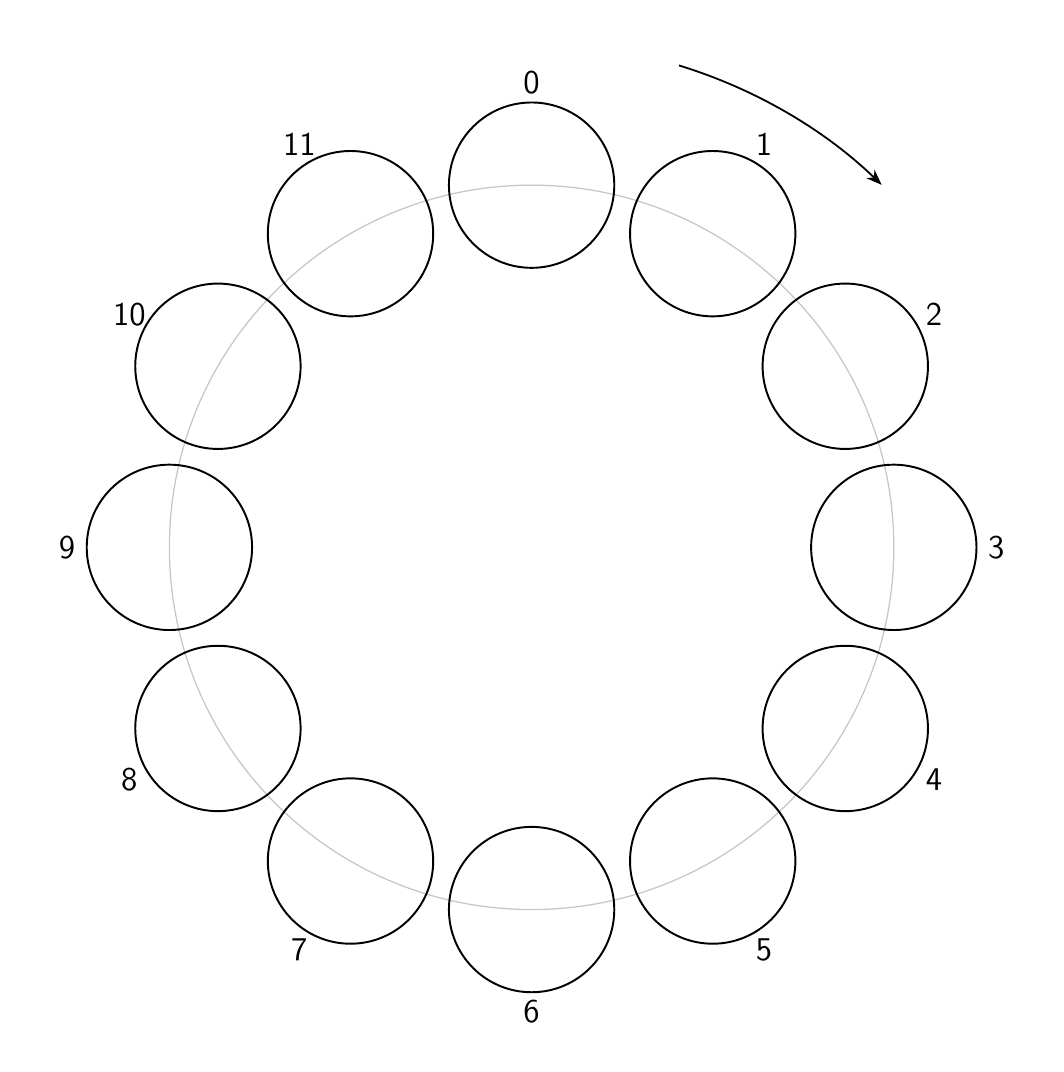
\begin{tikzpicture}[x=1mm,y=1mm]
  \path[use as bounding box] (-64,-63) rectangle (64,66);
  \draw[gray!45,line width=.45pt] (0,0) circle[radius=46];
  \foreach \i in {0,...,11}{
    \pgfmathsetmacro{\ang}{90-30*\i}
    \draw[line width=.7pt] (\ang:46) circle[radius=10.5];
    \node[font=\large] at (\ang:59) {\i};
  }
  \draw[arrow] (73:64) arc[start angle=73,end angle=46,radius=64];
\end{tikzpicture}}

\newcommand{\necklace}[2]{%
\begin{tikzpicture}[x=1mm,y=1mm]
  \path[use as bounding box] (-#1-4,-#1-4) rectangle (#1+4,#1+4);
  \draw[gray!45,line width=.4pt] (0,0) circle[radius=#1];
  \foreach \i in {0,...,5}{
    \pgfmathsetmacro{\ang}{90-60*\i}
    \draw[line width=.6pt] (\ang:#1) circle[radius=#2];
  }
\end{tikzpicture}}

\begin{document}
\textbf{Problem 1:} Each turn, red hops 2 circles clockwise and blue hops 5.
Move both before you check. They meet only if they land on the same circle.
Find the first meeting after at least one turn for each starting pair, if there is one.
Then choose another starting pair. Record landings as (red, blue).

\begin{center}
\begin{tikzpicture}[x=1mm,y=1mm]
  \path[use as bounding box] (0,-5) rectangle (176,17);
  \node[font=\small] at (17,14) {Before};
  \node[chip,draw=counterred,text=counterred] at (10,4) {11};
  \node[chip,draw=counterblue,text=counterblue] at (24,4) {6};
  \node[font=\small,text=counterred] at (79,10) {$11\to0\to1$};
  \node[font=\small,text=counterblue] at (79,1) {$6\to7\to8\to9\to10\to11$};
  \draw[arrow] (36,4) -- (45,4);
  \draw[arrow] (116,4) -- (126,4);
  \node[font=\small] at (145,14) {After one turn};
  \node[chip,draw=counterred,text=counterred] at (138,4) {1};
  \node[chip,draw=counterblue,text=counterblue] at (152,4) {11};
  \node[font=\small] at (145,-4) {$(1,11)$};
\end{tikzpicture}

\vspace{-2mm}
\workingring

\vspace{-2mm}
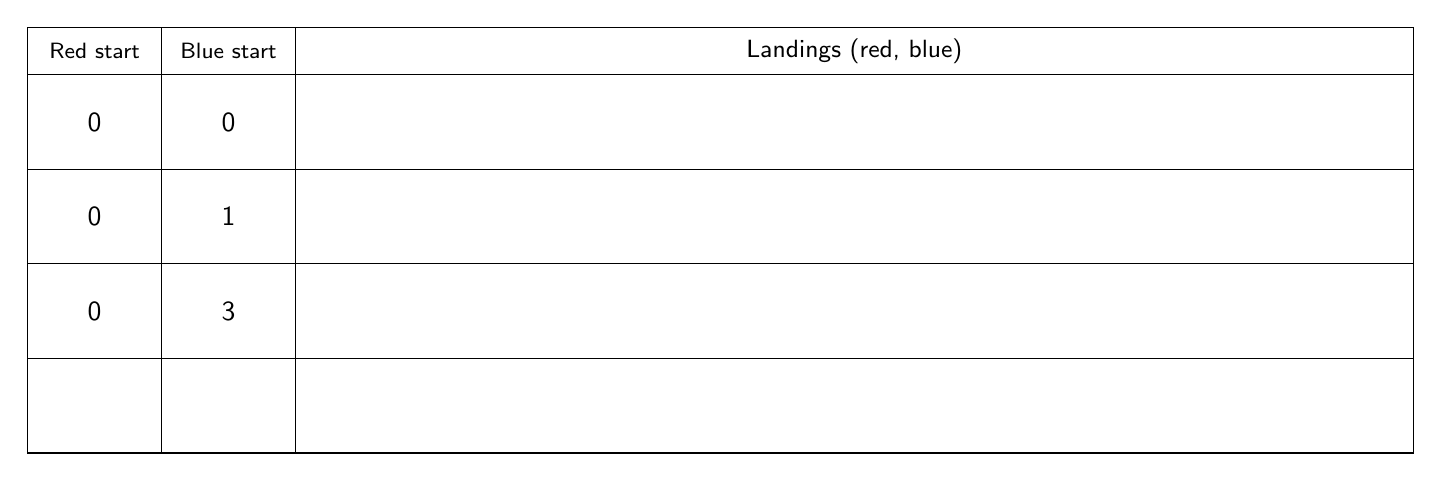
\begin{tikzpicture}[x=1mm,y=1mm]
  \path[use as bounding box] (0,0) rectangle (176,54);
  \draw[line width=.5pt] (0,0) rectangle (176,54);
  \foreach \x in {17,34}{\draw (\x,0)--(\x,54);}
  \foreach \y in {12,24,36,48}{\draw (0,\y)--(176,\y);}
  \node[font=\footnotesize] at (8.5,51) {Red start};
  \node[font=\footnotesize] at (25.5,51) {Blue start};
  \node[font=\small] at (105,51) {Landings (red, blue)};
  \node at (8.5,42) {0}; \node at (25.5,42) {0};
  \node at (8.5,30) {0}; \node at (25.5,30) {1};
  \node at (8.5,18) {0}; \node at (25.5,18) {3};
\end{tikzpicture}
\end{center}

\newpage
\textbf{Problem 2:} Start each route at 0. On each hop, choose either of the two allowed hop sizes
and move clockwise. Find the circles you can reach with each pair of hop choices.
Find shortest routes to 1 and to 2 whenever you can. Record a route by writing its hop sizes in order.

\begin{center}
\begin{tikzpicture}[x=1mm,y=1mm]
  \path[use as bounding box] (0,-5) rectangle (176,19);
  \foreach \x/\v in {10/0,47/4,84/8,121/11,158/3}{
    \node[chip] at (\x,9) {\v};
  }
  \foreach \x/\h in {10/4,47/4,84/3,121/4}{
    \draw[arrow] (\x+5,9)--(\x+31,9);
    \node[font=\small] at (\x+18.5,16) {hop \h};
  }
  \node[font=\small] at (84,-2) {Hop word: $4\quad4\quad3\quad4$};
\end{tikzpicture}

\vspace{-1mm}
\workingring

\vspace{-1mm}
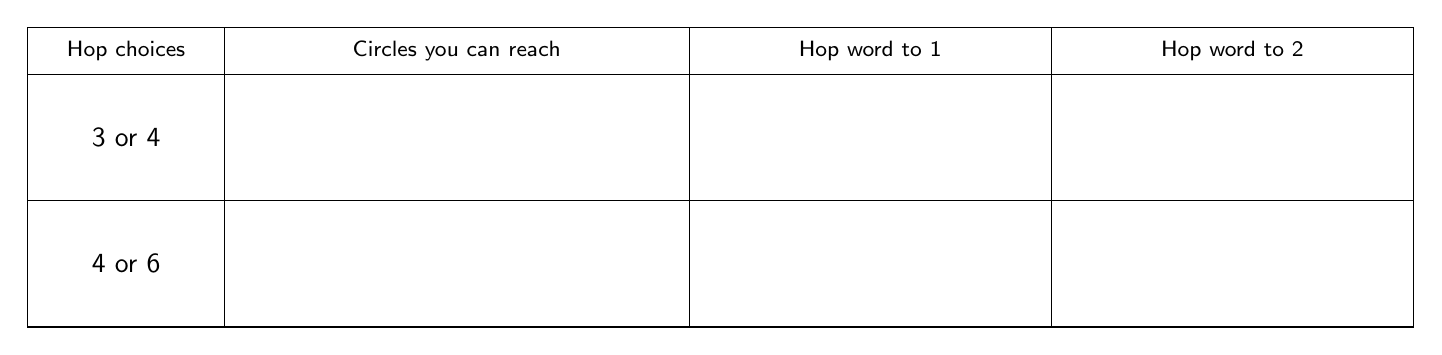
\begin{tikzpicture}[x=1mm,y=1mm]
  \path[use as bounding box] (0,0) rectangle (176,38);
  \draw[line width=.5pt] (0,0) rectangle (176,38);
  \foreach \x in {25,84,130}{\draw (\x,0)--(\x,38);}
  \draw (0,16)--(176,16); \draw (0,32)--(176,32);
  \node[font=\footnotesize] at (12.5,35) {Hop choices};
  \node[font=\footnotesize] at (54.5,35) {Circles you can reach};
  \node[font=\footnotesize] at (107,35) {Hop word to 1};
  \node[font=\footnotesize] at (153,35) {Hop word to 2};
  \node at (12.5,24) {3 or 4};
  \node at (12.5,8) {4 or 6};
\end{tikzpicture}
\end{center}

\newpage
\textbf{Problem 3:} Place 3 red and 3 blue counters on the large ring.
Two necklaces are the same if turning one ring while the other stays still makes them match.
Do not flip a ring over. Draw every different necklace on the small rings.
Which of your necklaces match themselves after a turn smaller than a full turn?

\begin{center}
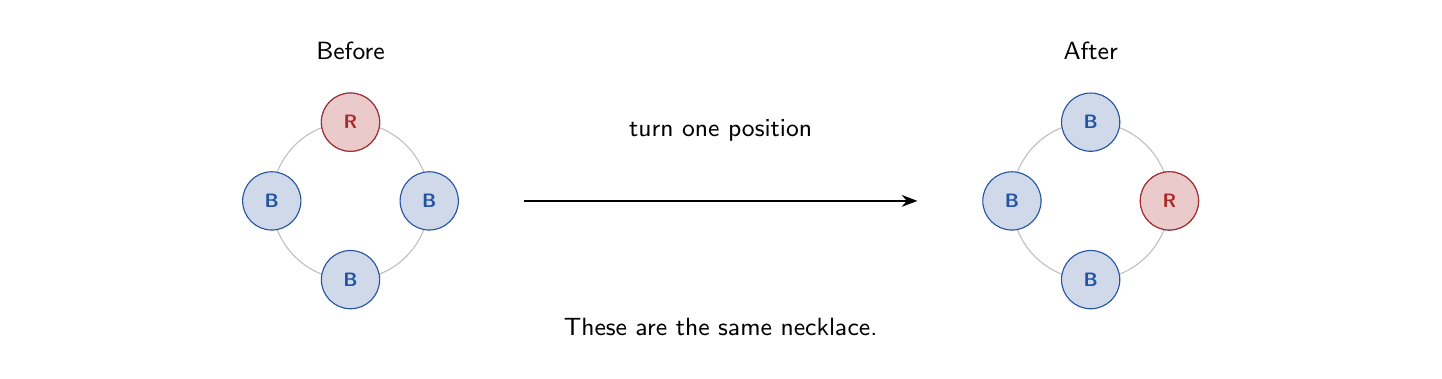
\begin{tikzpicture}[x=1mm,y=1mm]
  \path[use as bounding box] (0,-19) rectangle (176,22);
  \node[font=\small] at (41,19) {Before};
  \node[font=\small] at (135,19) {After};
  \foreach \cx in {41,135}{\draw[gray!50] (\cx,0) circle[radius=10];}
  \foreach \a in {0,90,180,270}{
    \draw[fill=counterblue!22,draw=counterblue] (41,0)++(\a:10) circle[radius=3.7];
    \draw[fill=counterblue!22,draw=counterblue] (135,0)++(\a:10) circle[radius=3.7];
  }
  \draw[fill=counterred!25,draw=counterred] (41,10) circle[radius=3.7];
  \draw[fill=counterred!25,draw=counterred] (145,0) circle[radius=3.7];
  \foreach \cx/\a in {41/90,135/0}{
    \node[text=counterred,font=\scriptsize\bfseries] at ({\cx+10*cos(\a)},{10*sin(\a)}) {R};
  }
  \foreach \a in {0,180,270}{\node[text=counterblue,font=\scriptsize\bfseries] at ({41+10*cos(\a)},{10*sin(\a)}) {B};}
  \foreach \a in {90,180,270}{\node[text=counterblue,font=\scriptsize\bfseries] at ({135+10*cos(\a)},{10*sin(\a)}) {B};}
  \draw[arrow] (63,0)--(113,0);
  \node[font=\small] at (88,9) {turn one position};
  \node[font=\small] at (88,-16) {These are the same necklace.};
\end{tikzpicture}

\vspace{-2mm}
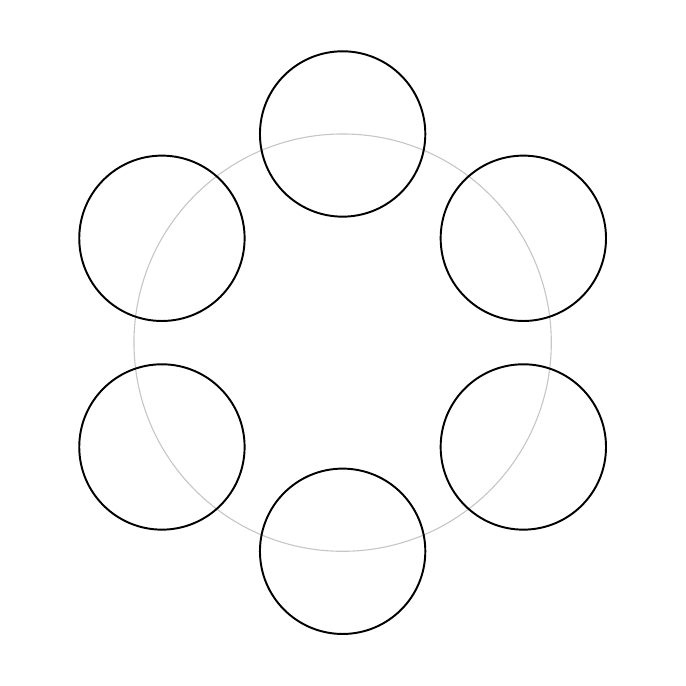
\begin{tikzpicture}[x=1mm,y=1mm]
  \path[use as bounding box] (-40,-40) rectangle (40,40);
  \draw[gray!45] (0,0) circle[radius=26.5];
  \foreach \i in {0,...,5}{
    \pgfmathsetmacro{\ang}{90-60*\i}
    \draw[line width=.7pt] (\ang:26.5) circle[radius=10.5];
  }
\end{tikzpicture}

\vspace{2mm}
\necklace{14}{3.5}\hspace{15mm}\necklace{14}{3.5}\hspace{15mm}\necklace{14}{3.5}

\vspace{5mm}
\necklace{14}{3.5}\hspace{15mm}\necklace{14}{3.5}\hspace{15mm}\necklace{14}{3.5}
\end{center}
\end{document}
